Finally, we introduce the empirical Fisher.
This matrix serves as an approximation to the type-I Fisher that does not require Monte Carlo samples.
Several contemporary optimizers, \eg the Adam variants, gained inspiration from second-order optimization, in particular preconditioning with the empirical Fisher.
For example, Adam \cite{kingma2015adam} stores the moving average of the mini-batch loss' squared gradients, which is motivated by (but is not equivalent to) preconditioning with the \emph{diagonal} of the empirical Fisher\footnote{See~\citet{lin2024can} for the exact preconditioner Adam approximates, which is a different approximation of the Fisher information matrix.}.
We obtain the empirical Fisher by replacing the model's likelihood in the type-I Fisher with the empirical likelihood, and evaluating the expectation over it:

\begin{definition}[Empirical Fisher (\Cref{basics/emp_fishers})]\label{def:emp_fisher}%
  The empirical Fisher matrix of the likelihood $\log r(\rvy \mid \vf_n)$,
  $\mE(\vtheta) \in \sR^{D \times D}$, is
  \begin{align*}
    & \mE(\vtheta) \\
	& = \frac{1}{N} \sum_{n}
	\begin{aligned}[t]
	   & (-\nabla_{\vtheta} \log r(\rvy = \vy_n \mid \vf_n))        \\
	   & (-\nabla_{\vtheta} \log r(\rvy = \vy_n \mid \vf_n))^{\top} \\
	\end{aligned} \\
    & = \frac{1}{N} \sum_{n}
    \begin{aligned}[t]
       & \left(\jac_{\vtheta}\vf_n\right)^{\top}                  \\
       & (-\nabla_{\vf_n} \log r(\rvy = \vy_n \mid \vf_n))        \\
       & (-\nabla_{\vf_n} \log r(\rvy = \vy_n \mid \vf_n))^{\top} \\
       & \jac_{\vtheta}\vf_n.
    \end{aligned}
  \end{align*}
\end{definition}

\switchcolumn[1]
\codeblock{basics/emp_fishers}
\codeblock{basics/emp_fisher_product}
\switchcolumn[0]

\Cref{basics/emp_fisher_product} implements multiplication with the EF.

\paragraph{Empirical Fisher $\neq$ Fisher.}
The subtle difference between empirical and type-I Fisher is the \emph{expectation} over the gradient outer product
\begin{align*}
  (-\nabla_{\vtheta} \log r(\rvy \mid \vf_n))
  (-\nabla_{\vtheta} \log r(\rvy \mid \vf_n))^{\top}
\end{align*}
\wrt the model's predictive distribution $r(\rvy \mid \vf_n)$, whereas $\mE(\vtheta)$ plugs in the \emph{ground-truth} labels $\vy_n$ into the gradient outer product.
While the computation of the empirical Fisher is more efficient than Monte Carlo approximating the type-I Fisher with number of samples $M > 1$, this subtle difference can impact the utility of this matrix in optimization.
In particular,~\citet{kunstner2019limitations} show that preconditioning with the EF can have detrimental effects in simple problems.
The empirical Fisher's success in some settings (\eg, through Adam) may be attributed to its ability to attenuate \emph{gradient noise}, not its properties as a curvature estimate.
To some extent, this is still an open question.

\paragraph{Visual comparison.} For our purposes, it suffices to acknowledge that the empirical Fisher is a popular curvature approximation is often used due to its computational advantages over the Fisher and GGN but differs from them, and can also be approximated using KFAC.
The differences between GGN, MC type-I Fisher, and empirical Fisher, as well as their variation under different flattening conventions, are visualized in \Cref{fig:visual-comparison-mc-empirical-fisher}.

\begin{figure}[!h]
  \centering
  \begin{minipage}[t]{0.49\linewidth}
    \centering
    $\cvec 1$ sample\vspace{1ex}
    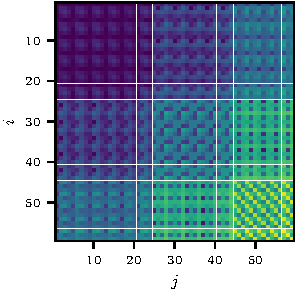
\includegraphics[width=1.0\linewidth]{../kfs/plots/synthetic_cvec_mcfisher_1.pdf}
  \end{minipage}
  \hfill
  \begin{minipage}[t]{0.49\linewidth}
    \centering
    $\rvec 1$ sample\vspace{1ex}
    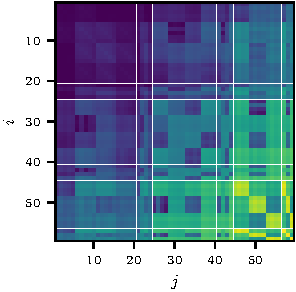
\includegraphics[width=1.0\linewidth]{../kfs/plots/synthetic_rvec_mcfisher_1.pdf}
  \end{minipage}
  \\
  \begin{minipage}[t]{0.49\linewidth}
    \centering
    $\cvec 100$ samples\vspace{1ex}
    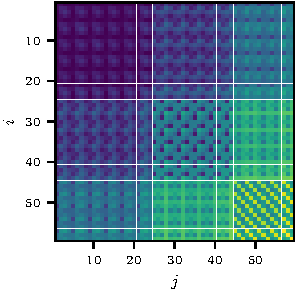
\includegraphics[width=1.0\linewidth]{../kfs/plots/synthetic_cvec_mcfisher_100.pdf}
  \end{minipage}
  \hfill
  \begin{minipage}[t]{0.49\linewidth}
    \centering
    $\rvec 100$ samples\vspace{1ex}
    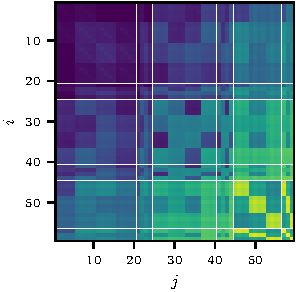
\includegraphics[width=1.0\linewidth]{../kfs/plots/synthetic_rvec_mcfisher_100.pdf}
  \end{minipage}
  \begin{minipage}[t]{0.49\linewidth}
    \centering
    $\cvec$ exact\vspace{1ex}
    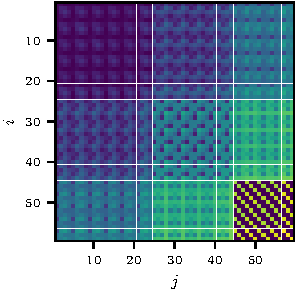
\includegraphics[width=1.0\linewidth]{../kfs/plots/synthetic_cvec_ggn.pdf}
  \end{minipage}
  \hfill
  \begin{minipage}[t]{0.49\linewidth}
    \centering
    $\rvec$ exact\vspace{1ex}
    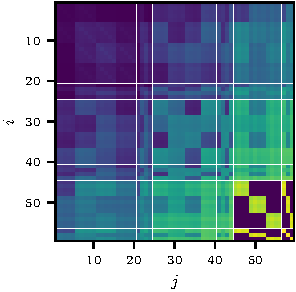
\includegraphics[width=1.0\linewidth]{../kfs/plots/synthetic_rvec_ggn.pdf}
  \end{minipage}
  \begin{minipage}[t]{0.49\linewidth}
    \centering
    $\cvec$ empirical\vspace{1ex}
    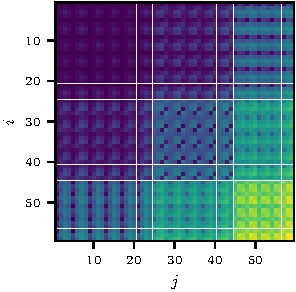
\includegraphics[width=1.0\linewidth]{../kfs/plots/synthetic_cvec_empfisher.pdf}
  \end{minipage}
  \hfill
  \begin{minipage}[t]{0.49\linewidth}
    \centering
    $\rvec$ empirical\vspace{1ex}
    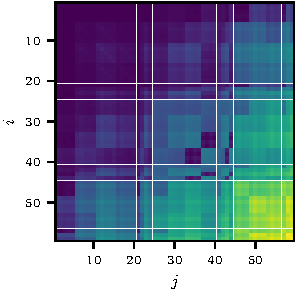
\includegraphics[width=1.0\linewidth]{../kfs/plots/synthetic_rvec_empfisher.pdf}
  \end{minipage}
  \caption{\textbf{Visual comparison of Fisher matrices.}
    The Fisher blocks are visually highlighted with white lines.
    The left column uses $\cvec$-flattening, the right column $\rvec$-flattening.
    The penultimate row uses the exact Fisher.
    The last row shows the empirical Fisher, highlighting its difference to the previous curvature estimates.
    The Fishers were evaluated on synthetic data ($N=100$) using an MLP with three fully-connected layers and ReLU activations (5-4-4-3) and square loss.
    Plots created with \repofile{plots/synthetic_fisher.py}.
  }\label{fig:visual-comparison-mc-empirical-fisher}
\end{figure}

%%% Local Variables:
%%% mode: LaTeX
%%% TeX-master: "../main"
%%% End:
